% Document setup
\documentclass[12pt]{article}
\usepackage[margin=1in]{geometry}
\usepackage{fancyhdr}
\usepackage{lastpage}

\pagestyle{fancy}
\lhead{Richard Whitehill}
\chead{PHYS 811 -- HW \HWnum}
\rhead{\duedate}
\cfoot{\thepage \hspace{1pt} of \pageref{LastPage}}

% Encoding
\usepackage[utf8]{inputenc}
\usepackage[T1]{fontenc}

% Math/Physics Packages
\usepackage{amsmath}
\usepackage{amssymb}
\usepackage{mathtools}
\usepackage{physics}
\usepackage{siunitx}

\AtBeginDocument{\RenewCommandCopy\qty\SI}

% Enumeration/itemize
\usepackage{enumitem}
\newenvironment{parts}
{\begin{enumerate}[label=\textbf{(\alph*)},leftmargin=*,itemsep=-10pt]
}{\end{enumerate}}

% Reference Style
\usepackage{hyperref}
\hypersetup{
    colorlinks=true,
    linkcolor=blue,
    filecolor=magenta,
    urlcolor=cyan,
    citecolor=green
}

\newcommand{\eref}[1]{Eq.~(\ref{eq:#1})}
\newcommand{\erefs}[2]{Eqs.~(\ref{eq:#1})--(\ref{eq:#2})}

\newcommand{\fref}[1]{Fig.~\ref{fig:#1}}
\newcommand{\frefs}[2]{Figs.~\ref{fig:#1}--\ref{fig:#2}}

\newcommand{\tref}[1]{Table~\ref{tab:#1}}
\newcommand{\trefs}[2]{Tables~\ref{tab:#1}-\ref{tab:#2}}

% Figures and Tables 
\usepackage{graphicx}
\usepackage{float}
\usepackage[font=small,labelfont=bf]{caption}

\newcommand{\bef}{\begin{figure}[h!]\begin{center}}
\newcommand{\eef}{\end{center}\end{figure}}

\newcommand{\bet}{\begin{table}[h!]\begin{center}}
\newcommand{\eet}{\end{center}\end{table}}

% tikz
\usepackage{tikz}
\usetikzlibrary{calc}
\usetikzlibrary{decorations.pathmorphing}
\usetikzlibrary{decorations.markings}
\usetikzlibrary{arrows.meta}
\usetikzlibrary{positioning}
\usetikzlibrary{3d}
\usetikzlibrary{shapes.geometric}

% tcolorbox
\usepackage[most]{tcolorbox}
\usepackage{xcolor}
\usepackage{xifthen}
\usepackage{parskip}

\newcommand*{\eqbox}{\tcboxmath[
    enhanced,
    colback=black!10!white,
    colframe=black,
    sharp corners,
    size=fbox,
    boxsep=8pt,
    boxrule=1pt
]}

% problem-solution macros
% \usepackage{adjustbox}
\usepackage{changepage}

\newtcolorbox{probbox}[1][]{
    breakable,
    enhanced,
    boxrule=0pt,
    frame hidden,
    borderline west={4pt}{0pt}{green!50!black},
    colback=green!5,
    before upper=\textbf{Problem #1) \,},
    % \textbf{Problem #1 \ifthenelse{\isempty{#1}}{}{: #1} \\ },
    sharp corners,
    parbox=false
}

% \newtcolorbox{ProblemBox}[1][]{%
%   breakable,
%   enhanced,
%   colback=black!10!white,
%   colframe=black,
%   title={\large #1 \hfill}
% }
\newcommand{\prob}[2]{
\begin{probbox}[#1]
#2
\end{probbox}
}

\newenvironment{solution}{\begin{adjustwidth}{8pt}{8pt}}{\end{adjustwidth}}
\newcommand{\sol}[1]{
\begin{solution}
#1
\end{solution}
}
% \textbf{#1)} #2}


% Listings

\definecolor{background}{RGB}{245,245,246}
\definecolor{rule}{RGB}{224,224,224}
\definecolor{keyword}{RGB}{0,128,0}
\definecolor{comment}{RGB}{172,191,206}

\lstdefinestyle{mystyle}{
    frame=trbl,
    basicstyle=\footnotesize,
    backgroundcolor=\color{background},
    rulecolor=\color{rule},
    commentstyle=\color{comment},
    keywordstyle=\color{keyword}\bfseries,
    keywordstyle={[2]\color{keyword}},
    numberstyle=\color{green},
    stringstyle=\color{red},
    showstringspaces=false,
    breakatwhitespace=false,
    breaklines=true,
    captionpos=b,
    keepspaces=true,
    numbersep=5pt,
    showspaces=false,
    showtabs=false,
    tabsize=2,
    columns=fixed,
}

\lstset{style=mystyle}

\lstnewenvironment{python}{
\lstset{
	language=Python,
	otherkeywords={as},
	emph={self},
	emphstyle=\color{Blue}
}
}
{}

\NewDocumentCommand{\inputpython}{m}{\lstinputlisting[language=Python]{#1}}


% Miscellaneous Definitions/Settings
\newcommand{\reals}{\mathbb{R}}
\newcommand{\integers}{\mathbb{Z}}
\newcommand{\naturals}{\mathbb{N}}
\newcommand{\rationals}{\mathbb{Q}}
\newcommand{\complexs}{\mathbb{C}}

\setlength{\parskip}{\baselineskip}
\setlength{\parindent}{0pt}
\setlength{\headheight}{14.49998pt}
\addtolength{\topmargin}{-2.49998pt}


\def\HWnum{5}
\def\duedate{November 25, 2024}


\begin{document}

\prob{1}{

Laplace's equation in 2D rectangular coordinates
\begin{align}
    \pdv[2]{f}{x} + \pdv[2]{f}{y} = 0
.\end{align}
The Laplace equation applies to problems in steady state heat conduction, ideal fluid flow, electrostatics, etc.
Write a code for solving 2D Laplace's equation using finite-difference $2^{\rm nd}$-order method and solve 2D Laplace's equation on the square $[0,h] \times [0,h]$ with $h = 10$ and the boundary conditions $f(x,0) = f(x,h) = f(0,y) = 0$ and $f(h,y) = 10$.

\begin{parts}
   
    \item Compute electric potential as a function of $x$ and $y$.

    \item Create a surface plot of the calculated potential.

    \item Run 10, 100, and 1000 iterations, and note when convergence occurs.

    \item Investigate the effect of varying the step size $\Delta h$.
        Draw conclusions regarding the stability and accuracy of the solution for various $\Delta h$.

    \item \textit{Optional}: Investigate the effect of using Gauss-Seidel relaxation versus Jacobi iterations.
        Which converges faster?

\end{parts}

}

\sol{

(a) We can discretize our space and convert this continuous partial differential equation into one relating the value of $f$ at neighboring lattice points using the finite difference method.
Letting $f(x_{i},y_{j}) = f_{i,j}$, we have
\begin{align}
    \frac{f_{i-1,j} - 2 f_{i,j} + f_{i+1,j}}{\Delta x^2} + \frac{f_{i,j-1} - 2 f_{i,j} + f_{i,j+1}}{\Delta y^2} = 0
.\end{align}
Rearranging, we have
\begin{align}
    f_{i,j} = \frac{1}{2} \Big( \frac{1}{\Delta x^2} + \frac{1}{\Delta y^2} \Big)^{-1} \Bigg[ \frac{f_{i-1,j} + f_{i+1,j}}{\Delta x^2} + \frac{f_{i,j-1} + f_{i,j+1}}{\Delta y^2} \Bigg]
.\end{align}
We can devise a method of relaxation based on this equation to construct a sequence for function values at each lattice point such that
\begin{align}
    f_{i,j}^{(n+1)} = \frac{1}{2} \Big( \frac{1}{\Delta x^2} + \frac{1}{\Delta y^2} \Big)^{-1} \Bigg[ \frac{f_{i-1,j}^{(n)} + f_{i+1,j}^{(n)}}{\Delta x^2} + \frac{f_{i,j-1}^{(n)} + f_{i,j+1}^{(n)}}{\Delta y^2} \Bigg]
,\end{align}
where we choose some initial configuration for $f^{(0)}$.
One can terminate the iteration after some chosen number of iterations or after an error tolerance is reached.


(b) In \fref{part1-comp} we plot the numeric solution in the left panel and the difference between the numeric and analytic solution\footnote{Note that contour plots are shown in this article instead of surface plots. There were some memory related issues that made creating the necessary surface plots problematic on my personal computer.}
\begin{align}
    \frac{V_{\rm analytic}(x,y)}{V_0} = \frac{4}{\pi} \sum_{n=1}^{\infty} \frac{1}{2n+1} \sin\Big( \frac{(2n+1) \pi x}{h} \Big) \frac{\sinh[(2 n + 1) \pi y / h]}{\sinh[(2n + 1) \pi]}
.\end{align}
We can see that for a sufficient relative tolerance as our termination condition in the iteration, the numeric solution is quite close to the analytic solution.
Note that if memory serves correctly, it may be possible to sum this series in closed form, in which case such a treatment would be discussed in \textit{Classical Electrodynamics} by Jackson.
For the code implementation here, there is some difficulty for large $n$ given that $\sinh(x)$ diverges when $x \rightarrow \infty$.
Thus, for to avoid overflow issues and a more efficient evaluation of such terms, it may be desirable to form an asymptotic series for the ratio of the hyperbolic sines in the numerator and denominator or find some other approach.


\begin{figure}[h!tb]
    \centering
    \includegraphics[width=\linewidth]{part1-comp.pdf}
    \caption{\textbf{Left}: Numeric solution for $N=50^2$ uniformly distributed points in $(x,y)$ grids with $V_0 = 10$ at $y = h$. \textbf{Right}: Absolute difference of the numeric and analytic series solution (evaluted for 100 terms).}
    \label{fig:part1-comp}
\end{figure}

(c) In \fref{part1-iter}, we show the results of the numeric iteration, running a maximum of $N = 10,100,1000$ relaxation iterations for the same configuration as in \fref{part1-comp}.
Note that none of the panels have converged to satisfy the relative error tolerance: it takes roughly 5000 iterations to do so.
However, we can see that our algorithm works as expected, which is that our configuration ideed is relaxing stably to the expected solution.

\begin{figure}[h!tb]
    \centering
    \includegraphics[width=\linewidth]{part1-iter.pdf}
    \caption{Numeric solutions for $N = 50^2$ uniformly distributed points in $(x,y)$ grids, run with a maximum number of iterations $10,100,1000$ from left to right, with $V_0 = 10$ at $y = h$.}
    \label{fig:part1-iter}
\end{figure}


(d) In \fref{part1-N}, we show the results of the numeric iteration, running on a different grid density with $N = 10^2,100^2,500^2$ uniformly spaced points a maximum of 30,000 iterations.
Although the algorithm is still stable and the first two configurations converge, the latter fails to in a small running time.
This is primarily because of the exponentially larger number of floating point operations.
In particular, the propagation of the boundary conditions to the interior of the square region requires a larger number of iterations.

\begin{figure}[h!tb]
    \centering
    \includegraphics[width=\linewidth]{part1-N.pdf}
    \caption{Numeric solutions for $N = 10^2,100^2,500^2$ uniformly distributed points in $(x,y)$ grids, from left to right, with $V_0 = 10$ at $y = h$.}
    \label{fig:part1-N}
\end{figure}


\inputpython{prob1.py}

}


\prob{2}{

Poisson's equation in 2D rectangular coordinates has a nonhomogeneous term
\begin{align}
    \pdv[2]{f}{x} + \pdv[2]{f}{y} = - 4 \pi \rho(x,y)
.\end{align}
Now consider the following boundary conditions for the square region $[0,h] \times [0,h]$ with $h = \pi$,
\begin{align}
\begin{gathered} 
    f(x,0) = \sin{x}, \quad f(x,h) = |\sin{2x}| \\
    f(0,y) = \frac{1}{2} \sin{y}, \quad f(h,y) = 1.2 \sin{y}
,\end{gathered}
\end{align}
and 
\begin{align}
    -4 \pi \rho(x,y) = 
    \begin{cases}
        360 & x = y = h/3 \\
        0 & {\rm otherwise}
    \end{cases}
.\end{align}

\begin{parts}

\item Compute electric potential as a function of $x$ and $y$.

\item Create a surface plot of the calculated potential.

\item Investigate the effect of varying the step size $\Delta h$.
    Draw conclusions regarding the stability and accuracy of the solution for various $\Delta h$.

\end{parts}

}


\sol{

In this problem, we can utilize the same method of relaxation as in problem 1.
We need only add the source term such that
\begin{align} 
    f_{i,j}^{(n+1)} = \frac{1}{2} \Big( \frac{1}{\Delta x^2} + \frac{1}{\Delta y^2} \Big)^{-1} \Bigg[ \frac{f_{i-1,j}^{(n)} + f_{i+1,j}^{(n)}}{\Delta x^2} + \frac{f_{i,j-1}^{(n)} + f_{i,j+1}^{(n)}}{\Delta y^2} + 4 \pi \rho_{i,j} \Bigg]
.\end{align}


(b,c) In \fref{part2-N}, we plot results for the boundary conditions above.
Additionally, we suppose that the goal of the charge distribution was to simulate a point charge.
In order to make a better test function, we choose a new charge density modeled as
\begin{align}
    \rho(\vb*{x};\vb*{x}_{0},\sigma) = \frac{1}{\pi \sigma^2} e^{-(\vb*{x} - \vb*{x}_{0})^2 / (2 \sigma^2)}
,\end{align}
where $\vb*{x}_{0}$ and $\sigma$ are the center of the charge distribution and $\sigma$ being the spread of the charge.
As $\sigma \rightarrow 0$, $\rho(\vb*{x};\vb*{x}_{0}) \rightarrow \delta(\vb*{x} - \vb*{x}_{0})$.
The primary issue of the original charge distribution is that it is unphysical in that it has a value at a certain point, but has no measure and therefore leads to no total charge when integrated.
Additionally, in order to get any contribution from the original proposed charge distribution, one of the grid points must coincide with the ``charge'' location.
By replacing this with a Gaussian, we smear out the effects so that points near the center feel the effects more and those farther from the center feel them less, which replicates our physical intuition for a point charge distribution.

As we observed in problem (1), one can see the effects of increasing the grid size.
At the lower end of the range, our solution has converged, but the grid is not capable of capturing the rich variance provided by our boundary conditions and the existence of a charge, and at the higher end of the range, while our grid is capable of capturing the behavior of our potential, it is expensive to reach such a distribution on a personal computer.
In the middle of these values, though, we achieve a stable solution within a reasonable number of iterations.

\begin{figure}[h!tb]
    \centering
    \includegraphics[width=\linewidth]{part2-N.pdf}
    \caption{Potential satisfying Poisson's equation on a square region with a point charge located at $(x,y) = (h/3,h/3)$ and represented by a Gaussian of width $\sigma = 0.05$ (in arbitrary units).}
    \label{fig:part2-N}
\end{figure}


\inputpython{prob2.py}

}


\prob{3}{

The heat equation for 1D case is
\begin{align}
    \pdv{T(x,t)}{t} = a \pdv[2]{T(x,t)}{x}
.\end{align}
You are given a metal bar of length $L = 1~{\rm m}$ and aligned along the $x$-axis.
It is insulated along its length though not at its ends.
Initially the entire bar is at a uniform temperature of $T_0 = 100^{\circ}{\rm C}$ and then both ends are placed in contact with ice water at $0^{\circ}{\rm C}$.
Heat flows through the non-insulated ends only.

\begin{parts}

\item Write a code for solving $1D$ diffusion equation.

\item Calculate how the temperature varies along the length of the bar as a function of time.

\item Create a 3D plot of $T(x,t)$.

\item Vary the time and space steps in your calculation so that you obtain solutions that are stable in time and vary smoothly in both space and time.

\item Test what happens when the von Neumann stability condition $a \Delta t / \Delta x^2 \leq 0.5$ is not satisfied.

\item \textit{Optional}: The diffusion equation above can be solved analytically as series.
    Compare the analytic and numeric solutions.

\end{parts}

}

\sol{

(a) Following the same logic as the previous two problems, we discretize our space and use the finite difference method to write
\begin{align}
    T_{i,j+1} = T_{i,j} + \frac{a \Delta t}{\Delta x^2} \Big( T_{i-1,j} - 2 T_{i,j} + T_{i+1,j} \Big)
,\end{align}
where $T_{i,j} \equiv T(x_{i},t_{j})$.
With this, we already have a natural time-sequence from this equation given that $T(x,0)$ is supplied as well as the boundary conditions.

(b,c,d,f) In \fref{part3-sol-stable}, we have simulated the dynamical behavior of the temperature of the bar for the given initial configuration on a lattice of 100 points with $a = 1$ (in arbitrary units) and $\beta = 0.25$, where $\beta = a \Delta t / \Delta x^2$.
From the plot, we can see the expected behavior, which is that the temperature decreases throughout the bar, converging to the temparature of the ends, and that the temperature in the center of the bar decreases slower than those closer to the ends as expected.
We also have plotted the difference between the numeric and analytic solution, given by
\begin{align}
    T(x,t) = \frac{4 T_0}{\pi} \sum_{n=1}^{\infty} \frac{1}{2n+1} e^{- a (2n+1)^2 \pi^2 t / h^2} \sin(\frac{(2 n + 1) \pi x}{h})
.\end{align}
As opposed to the Laplace's equation analytic solution's $y$-dependence, there is no difficulty in implementing the time dependence given that here, the time dependence kills off the higher-``energy'' modes.


\begin{figure}[h!tb]
    \centering
    \includegraphics[width=\linewidth]{part3-sol.pdf}
    \caption{Solution to the heat diffusion equation with $T_0 = 100$ (in arbitrary units), $T = 0$ for all $t$ at the endpoints, and with $100$ grid points and $\beta = 0.25$.}
    \label{fig:part3-sol-stable}
\end{figure}


(f) In \fref{part3-sol-unstable}, we plot the result of the finite difference method with $\beta = 0.51$, which violates the von Neumann stability condition, and very clearly, we can see that the numerics are incredibly poorly behaved.
Indeed, the instability propagates through each successive step, leaving us at the last step in a place very far from the desired solution and initial configuration.

\begin{figure}[h!tb]
    \centering
    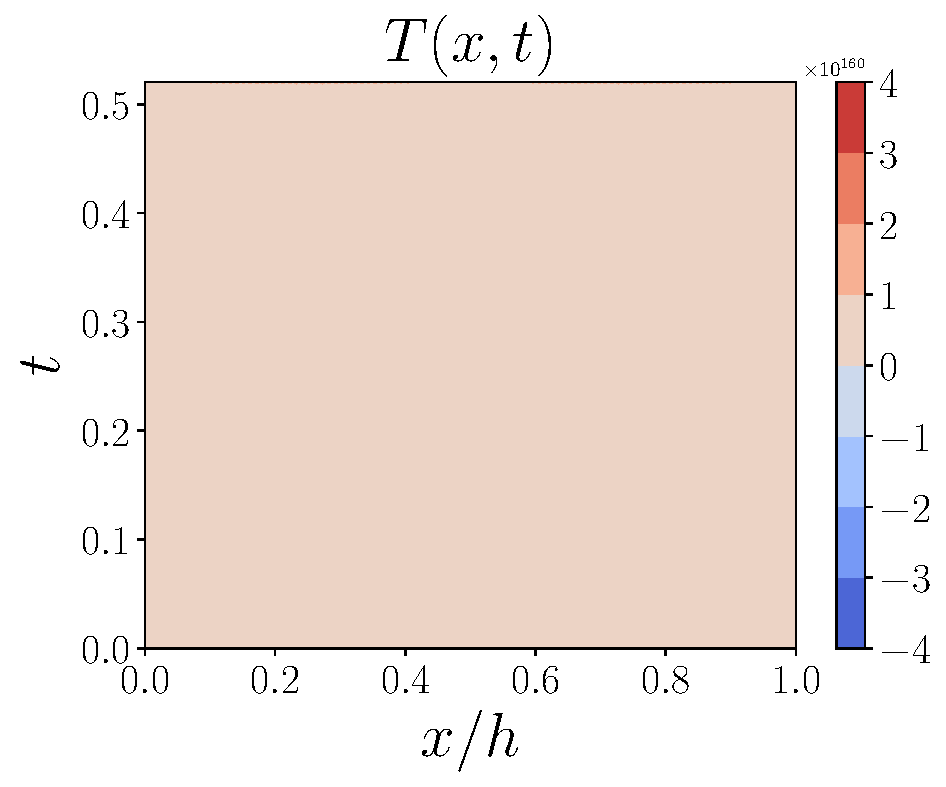
\includegraphics[width=0.5\linewidth]{part3-sol_unstable.pdf}
    \caption{Demonstration of the instability of the finite difference method when the von Neumann condition $\beta = a \Delta t / \Delta x^2 \leq 0.5$ is not satisfied.}
    \label{fig:part3-sol-unstable}
\end{figure}


\inputpython{prob3.py}


}


    
\end{document}
